\chapter{Свойства многослойных сферических маскирующих
  покрытий} \label{chapt3}

TODO перестновки в пространстве для хаотического дизайна.

\underline{\textbf{Третья глава}} посвящена исследованию свойств
многослойных сферических маскирующих покрытий. Схематическое
изображение модели приводится на рисунке~\ref{img:scattering}а. Для
заданного соотношения длины волны и диаметра маскируемого объекта с
помощью оптимизатора подбирались параметры многослойного покрытия
таким образом, чтобы уменьшить полное сечение рассеяния.  Покрытие
разбивалось на фиксированное количество слоёв одинаковой толщины, а в
качестве параметров оптимизации использовались показатели преломления
каждого слоя.  Результат оптимизации в виде зависимости полного
сечения рассеяния от количества слоёв и общей толщины покрытия
приводится на рисунке~\ref{img:scattering}б.
\begin{figure}[t]
  \begin{minipage}[ht]{0.45\linewidth}        
    \center{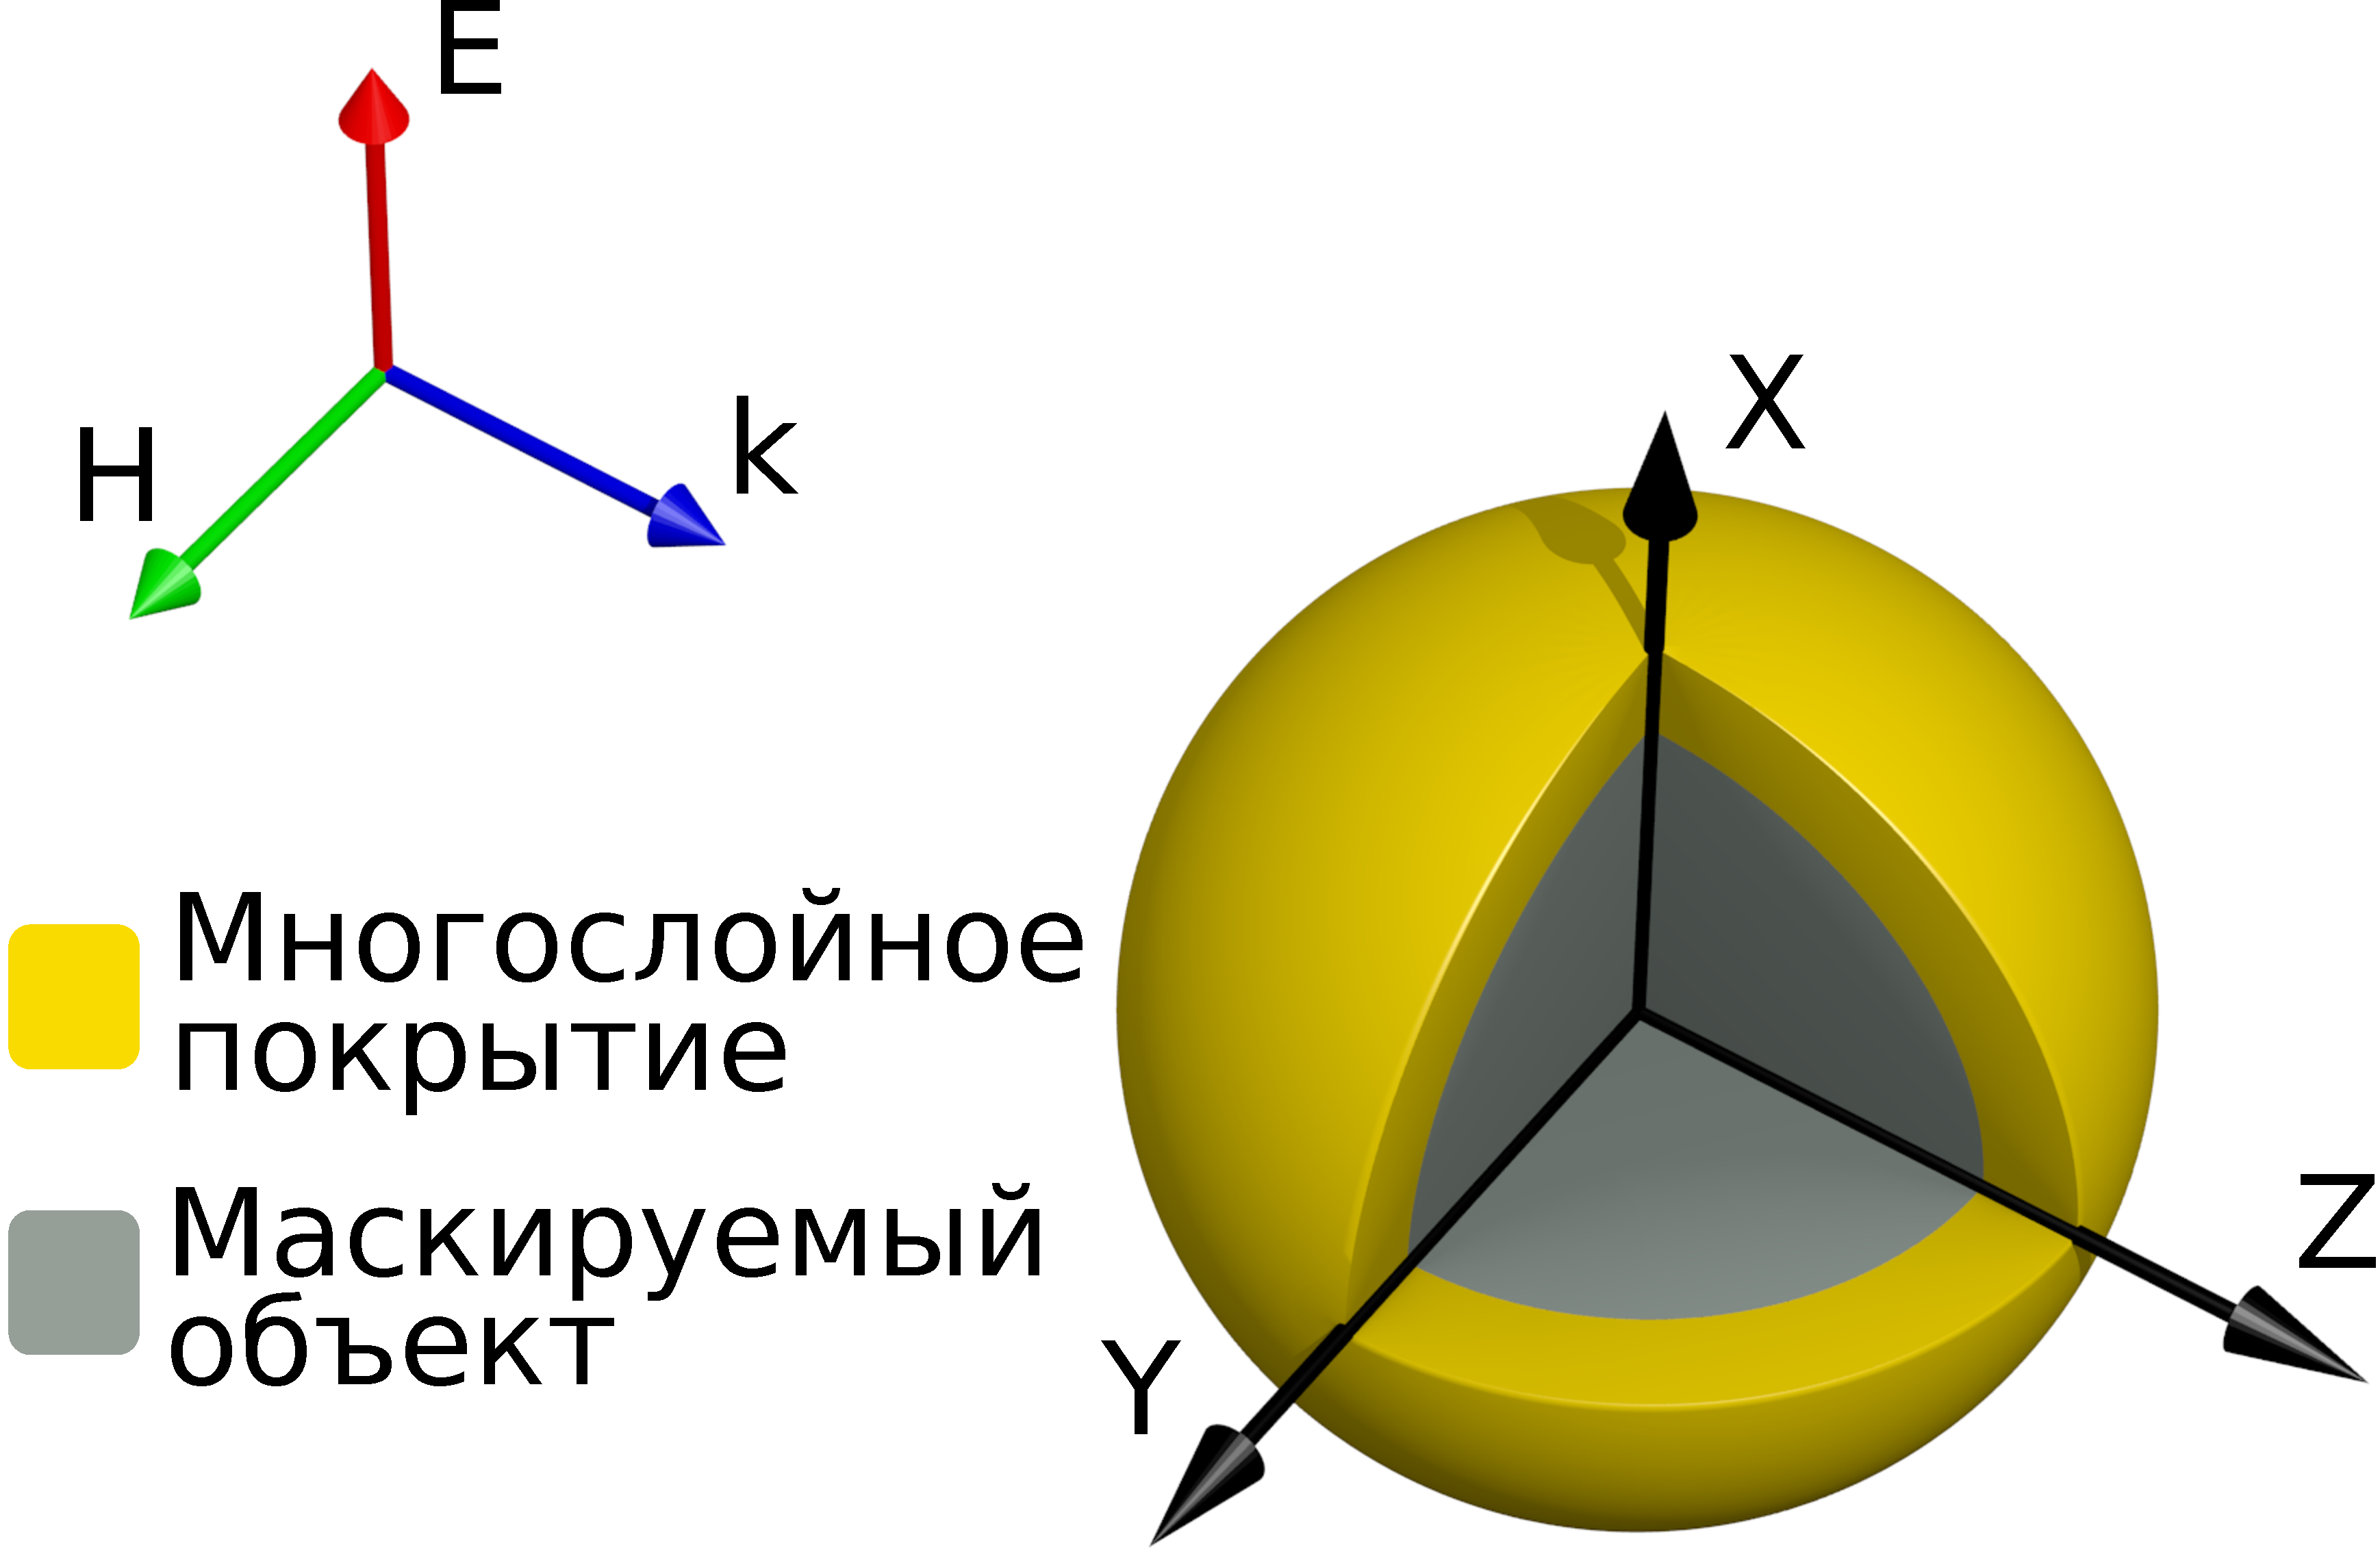
\includegraphics[width=0.95\linewidth]{model-view}}
  \end{minipage}
  \hfill
  \begin{minipage}[ht]{0.54\linewidth}
    \center{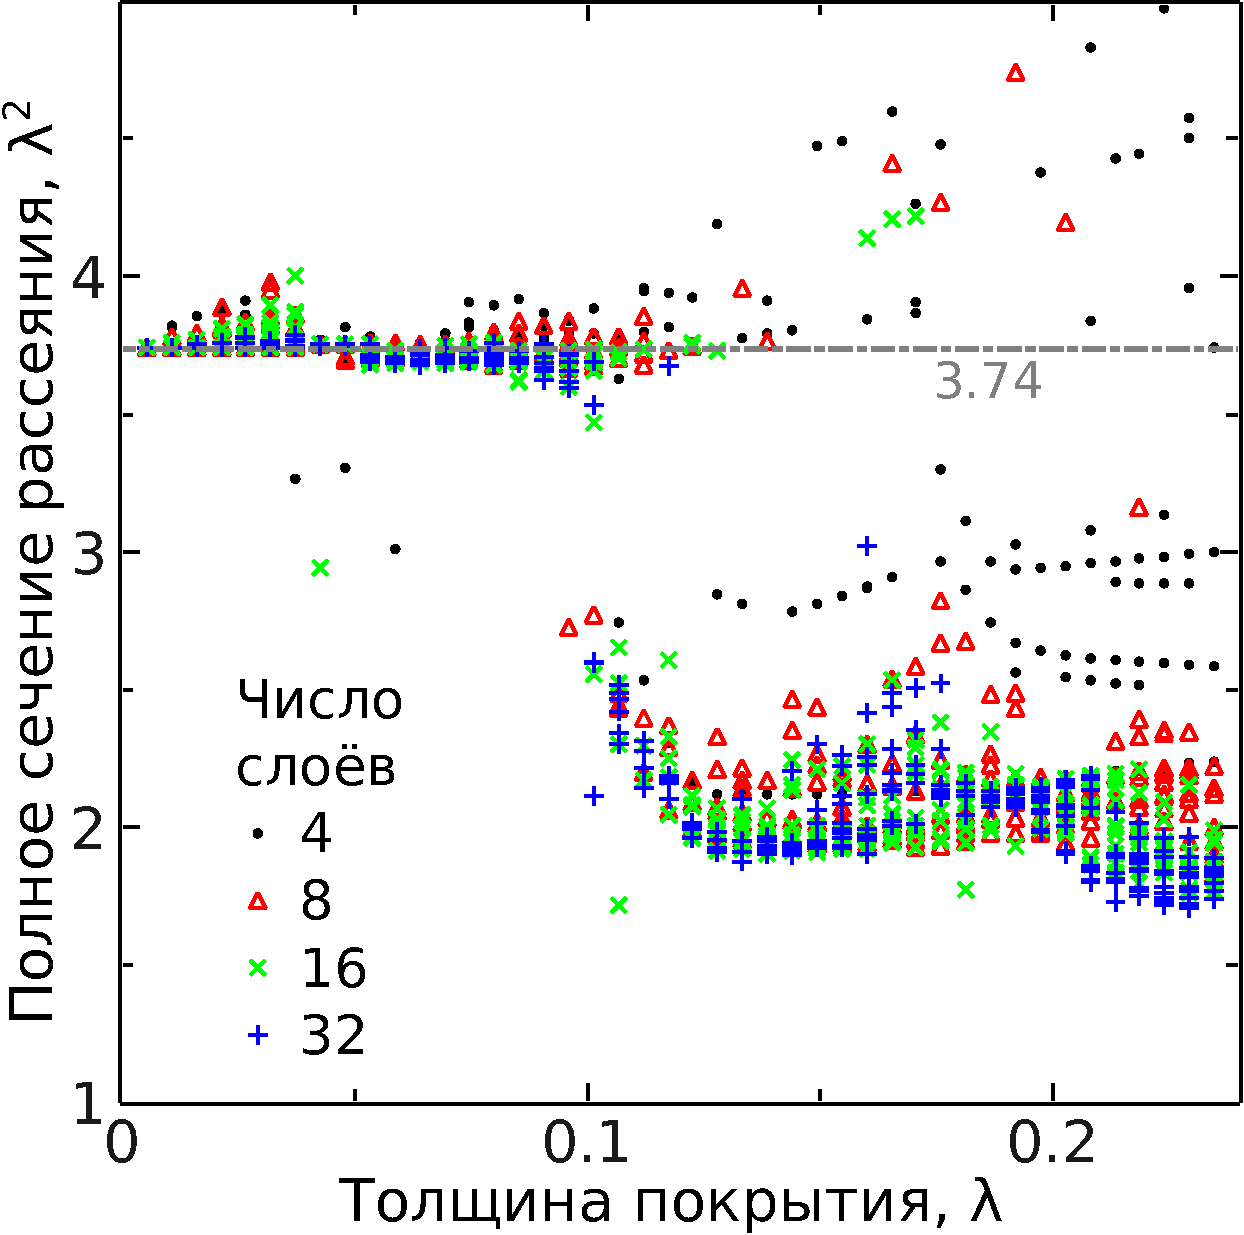
\includegraphics[width=0.95\linewidth]{rcs-overview} }
  \end{minipage}\\
  \vspace{0.3em}\\
  \begin{minipage}[ht]{0.45\linewidth}        
    \center{а)}
  \end{minipage}
  \hfill
  \begin{minipage}[ht]{0.54\linewidth}
    \center{б)}
  \end{minipage}

  \caption{(a) Схематическое изображение изучаемой системы: маскируемый
    объект -- сфера из идеального проводящего материала внутри
    многослойного диэлектрического покрытия и падающая
    электромагнитная волна. (б) 
    Результат работы оптимизатора для объекта диаметром $1.5\lambda$.
    % (TODO use plot for $\lambda/1.5$?)
    Каждая отметка на графике соответствует одному дизайну покрытия,
    полученному в результате минимизации рассеяния. При толщине
    покрытия $>0.15\lambda$ рассеяние можно уменьшить в $\sim 2$
    раза.}
  \label{img:scattering}  
\end{figure}
\begin{figure}[p]
  \begin{minipage}[ht]{0.32\linewidth}
    \center{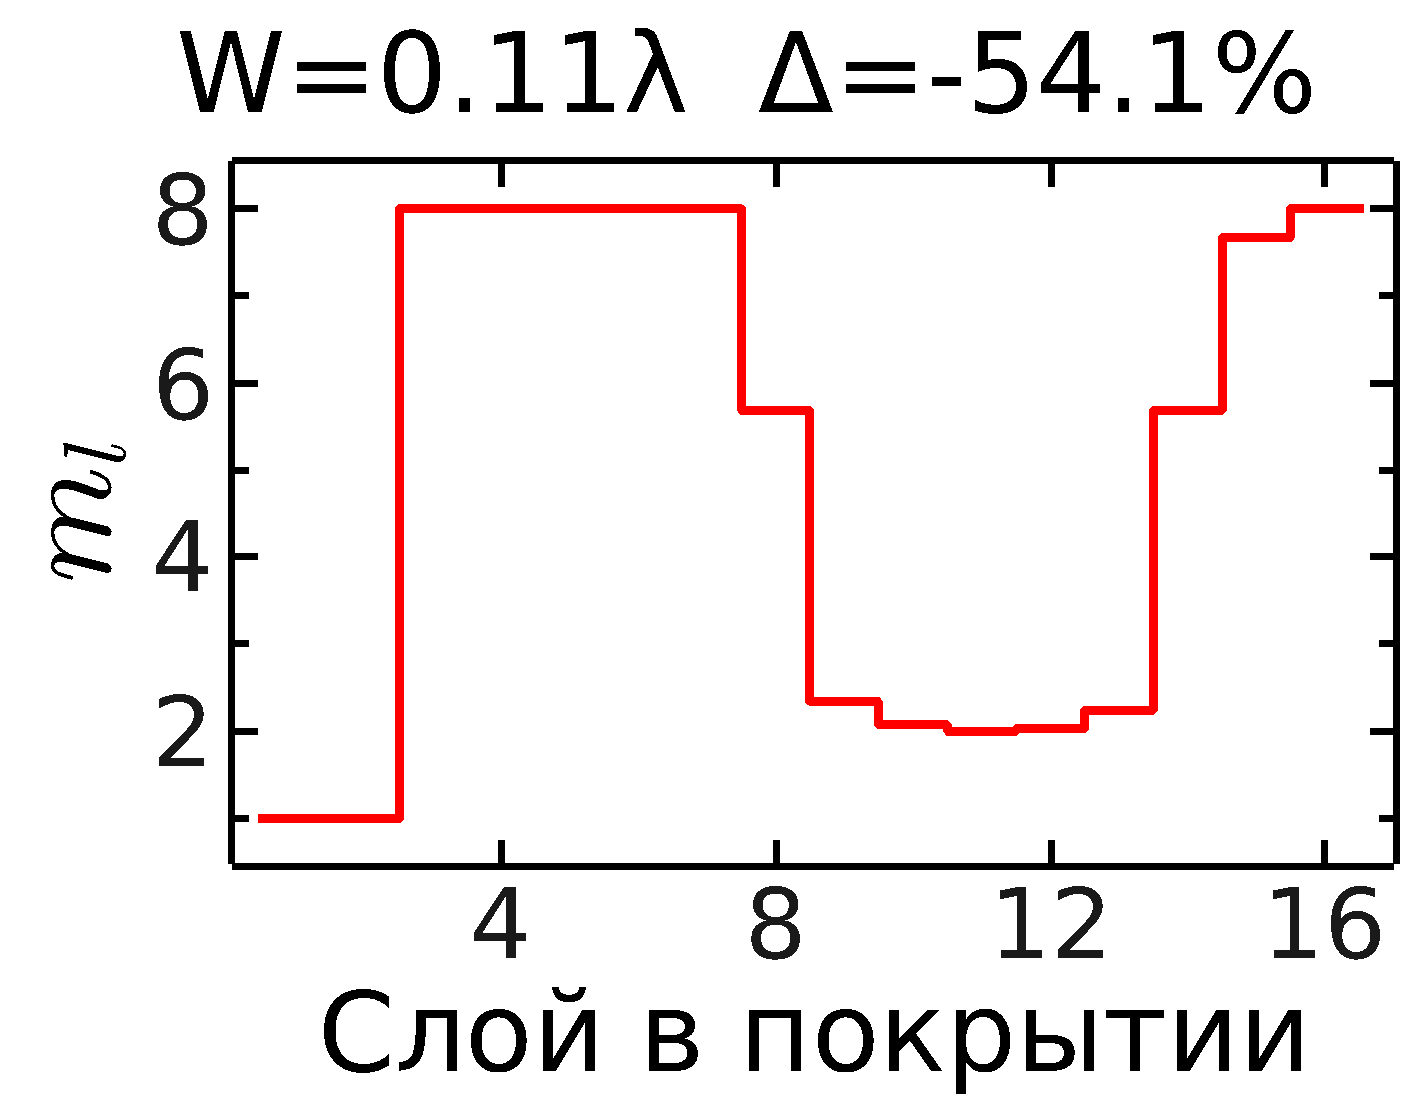
\includegraphics[width=0.95\linewidth]{w04-single-valley-index} \\ а)}
  \end{minipage}
  \hfill
  \begin{minipage}[ht]{0.32\linewidth}
    \center{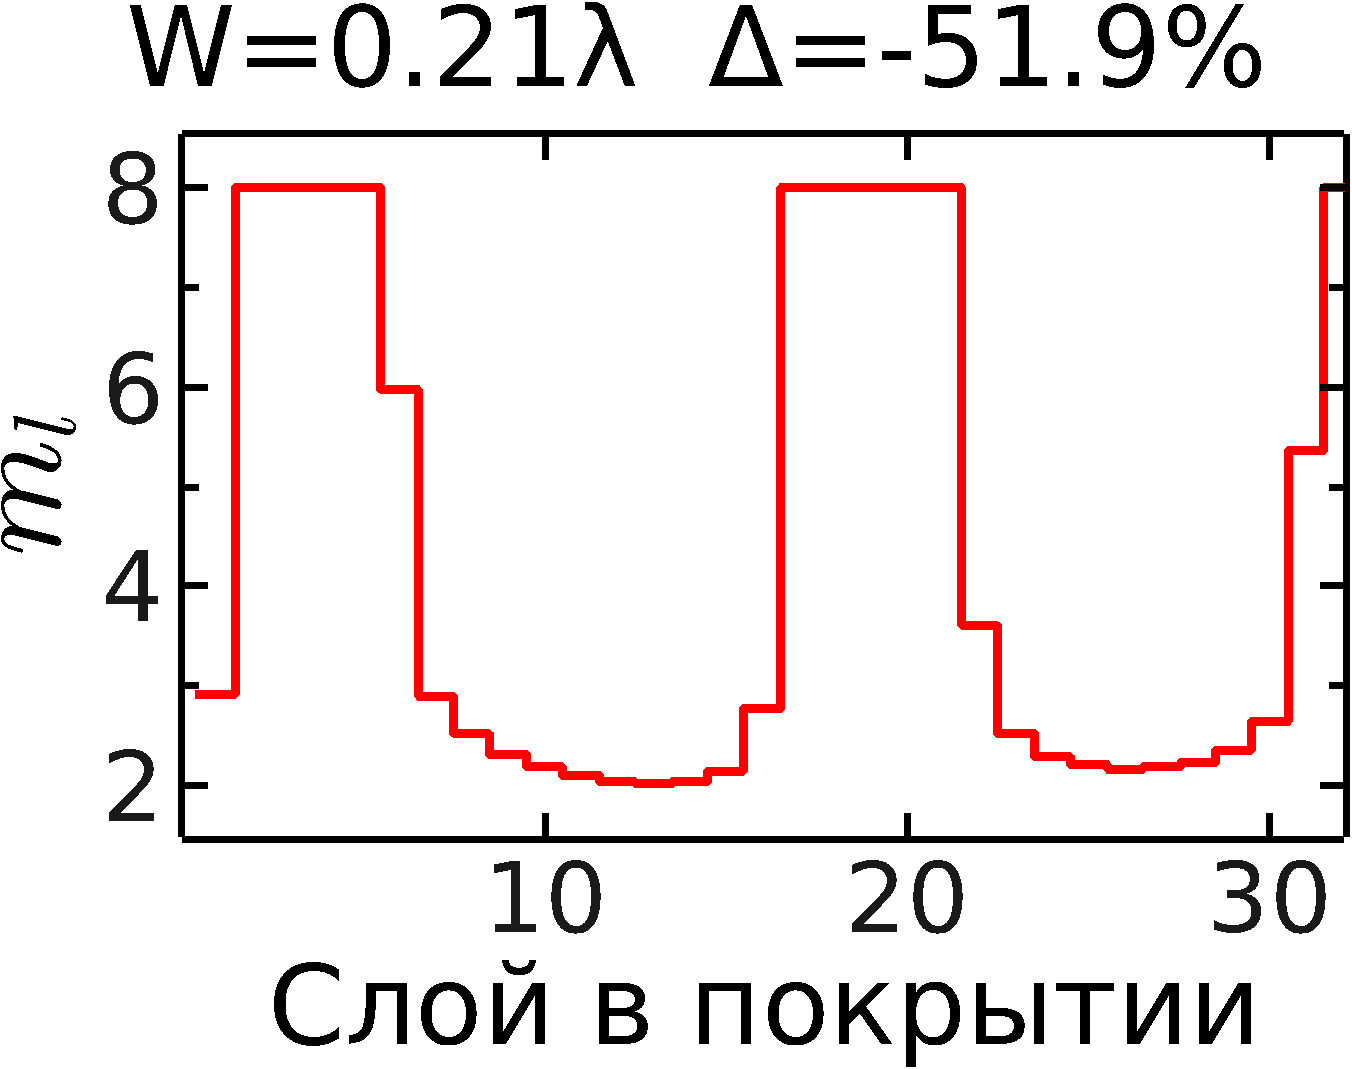
\includegraphics[width=0.95\linewidth]{w08-double-valley-index} \\ б)}
  \end{minipage}
  \hfill
  \begin{minipage}[ht]{0.32\linewidth}
    \center{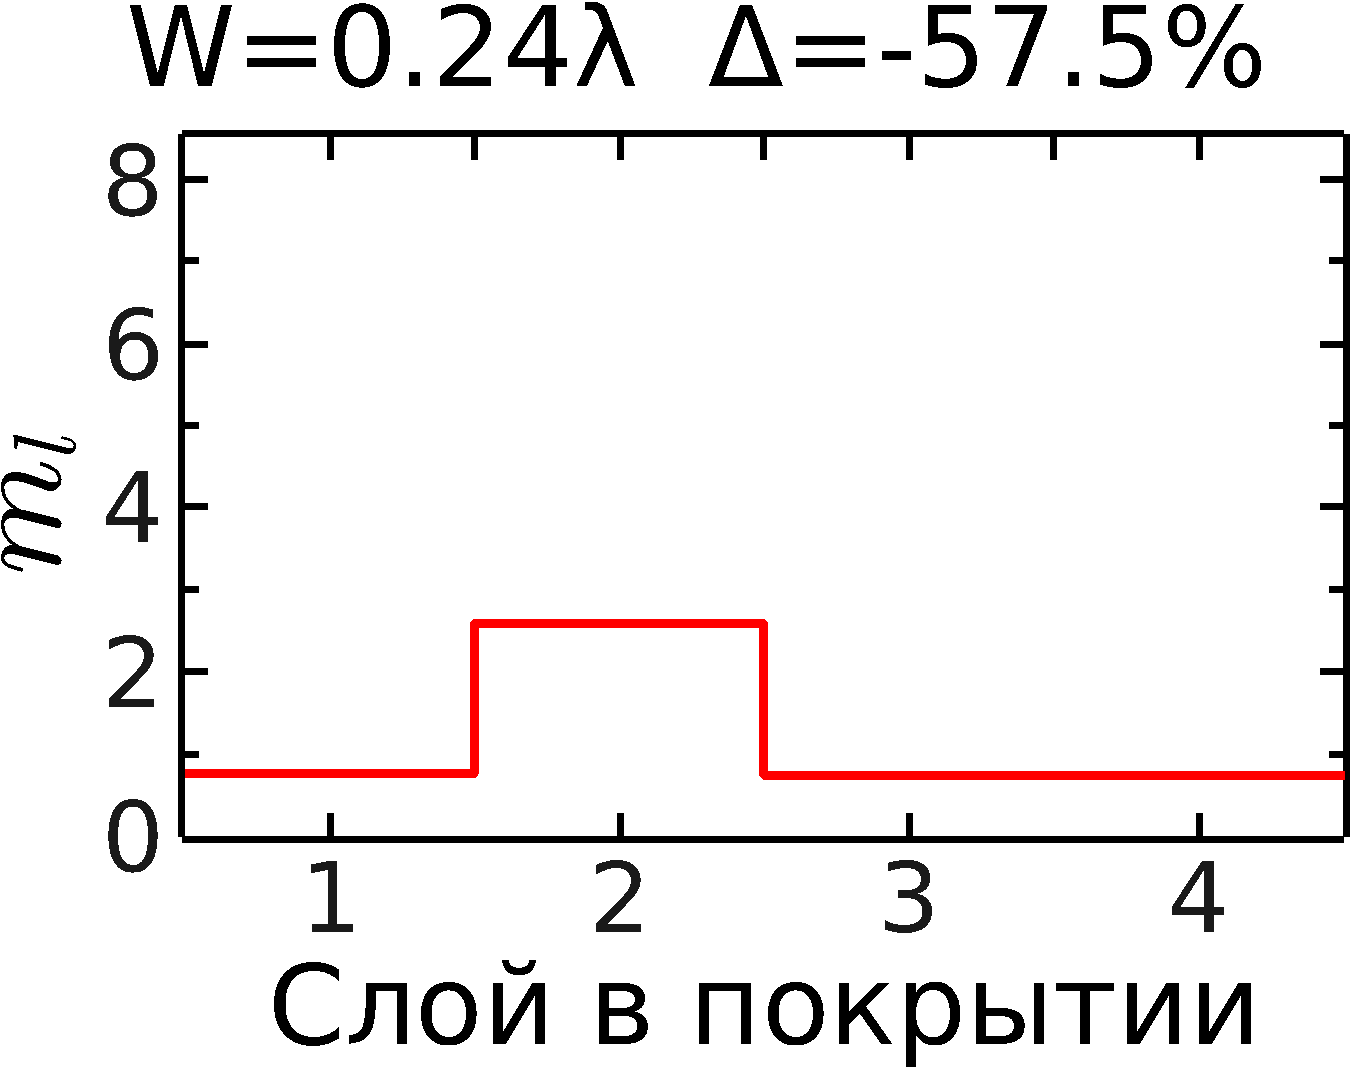
\includegraphics[width=0.95\linewidth]{index07-TO} \\ в)}
  \end{minipage}
  \caption{Типичные дизайны, обеспечивающие наилучшую маскировку при
    толщине покрытия, равной (a)~$0.11\lambda$, (б)~$0.21\lambda$ и
    (в)~$0.24\lambda$. Максимальное значение показателя преломления
    было ограничено $n_{\mathrm{max}}=8$, а минимальное значение
    было равно (а,б) $n_{\mathrm{min}}=1$ и (в) $n_{\mathrm{min}}=0.67$
  }
  \label{img:designs}  
\end{figure}
\begin{figure}[p]
  \begin{minipage}[ht]{0.495\linewidth}
    \center{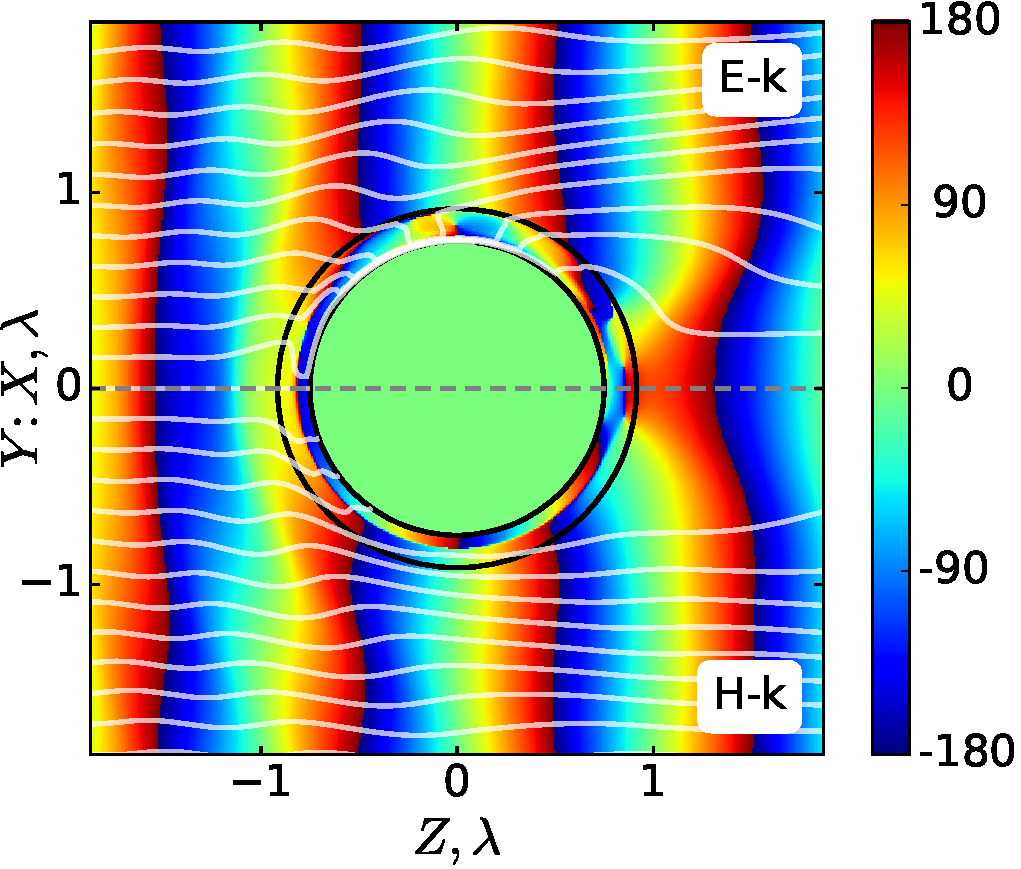
\includegraphics[width=0.98\linewidth]{PEC-index-sv-R3-XYZ-angleEx} \\ а)}
  \end{minipage}
  \hfill
  \begin{minipage}[ht]{0.495\linewidth}
    \center{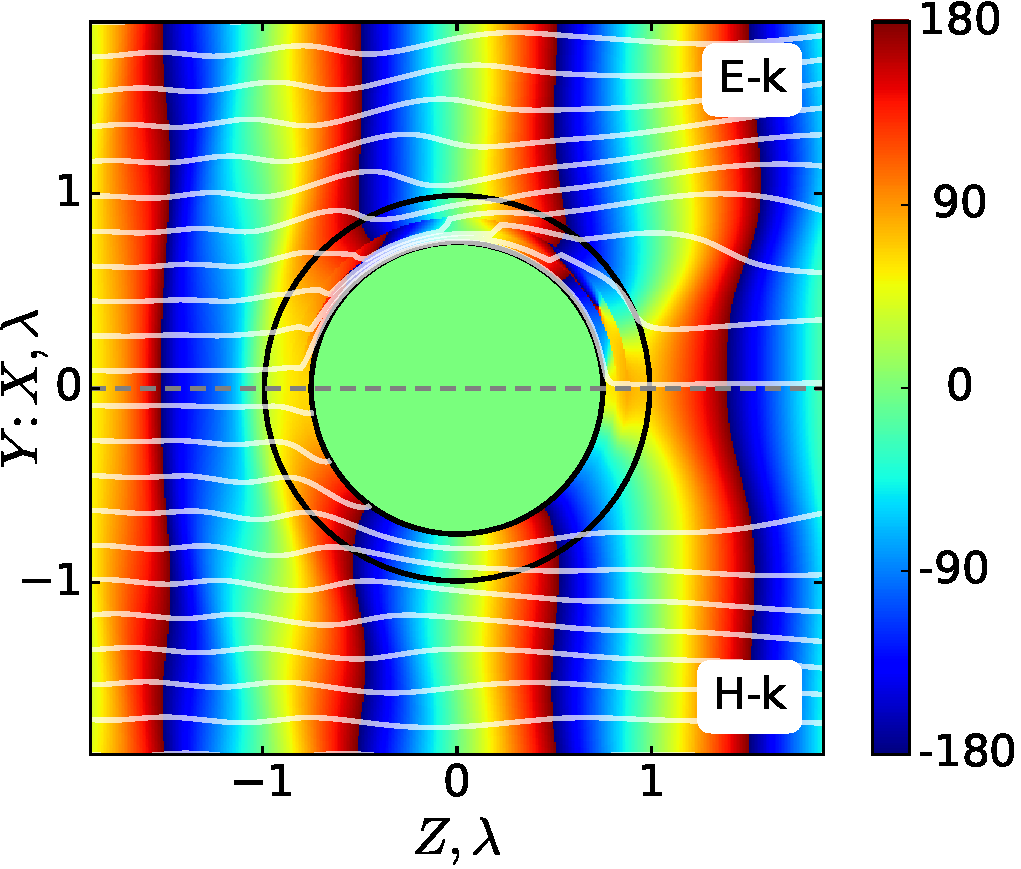
\includegraphics[width=0.98\linewidth]{PEC-index-in-glass-R1-XYZ-angleEx} \\ б)}
  \end{minipage}
  \caption{Изображение фазы электрического поля в случае маскировки
    объекта покрытием из изотропных (а) диэлектриков
    (см.~рисунок~\ref{img:designs}а) и (б) материалов с
    ${\varepsilon <1}$ (см.~рисунок~\ref{img:designs}в). Изображения
    построены в виде эпюра из плоскости поляризации падающей волны
    (верхняя половина) и перпендикулярной плоскости (нижняя
    половина). Чёрные окружности маркируют границы маскирующего
    покрытия. Белым обозначены линии потока энергии, волна
    распространяется в плоскости рисунка слева направо.}
  \label{img:field-phase}  
\end{figure}

Анализ этого и аналогичных графиков для других значений отношения
радиуса к длине волны позволил выявить ряд характерных
особенностей. Например, существует некое пороговое значение толщины,
после которого становится возможным стабильное получение дизайнов,
обеспечивающих заметное уменьшение сечения рассеяния. При этом
наилучшие показатели обеспечивают дизайны характерной структуры, где
несколько слоёв с высоким показателем преломления окружают группу
слоёв с низким показателем преломления. Увеличение общей толщины
покрытия приводит к переходу от дизайнов в одной такой группой
(рисунок~\ref{img:designs}а) к дизайнам с двумя группами
(рисунок~\ref{img:designs}б).

% ГОСТ Р 7.0.11—2011
% 5.3.9 На все иллюстрации должны быть приведены ссылки в тексте
% диссертации. При ссылке следует писать слово «Рисунок» с указанием
% его номера.

Сильной стороной теории Ми является возможность получать распределение
электрического и магнитного поля как внутри, так и вокруг изучаемой
наночастицы, вычислять значение фазы полей, а также строить линии
потока энергии.  Например, для структуры, изображённой на
рисунке~\ref{img:designs}а, было рассчитано распределение фазы
электрического поля в окружающем частицу пространстве и внутри
покрытия (рисунок~\ref{img:field-phase}а).  Из рисунка видно, что
волна, проходящая через маскирующее покрытие, испытывает задержку фазы,
приблизительно равную $2\pi$. Другими словами, такой дизайн приводит к
тому, что электромагнитная волна после распространения внутри покрытия
на выходе оказывается в фазе с волной, которая двигалась в окружающем
пространстве.  Это, в свою очередь, подавляет картину интерференции в
дальнем поле и, в конечном итоге, объясняет возникающий маскирующий
эффект.

Иначе выглядит распределение фазы электрического поля на
рисунке~\ref{img:field-phase}б, тут волна внутри покрытия на всей его
протяжённости движется в фазе с волной в окружающем пространстве. Это
стало возможным из-за использования в оптимизации материалов с
${\varepsilon<1}$, что соответствует маскировке объекта во вмещающей
среде, в которой скорость распространения света ниже, чем внутри
маскирующего покрытия.  Такие покрытия отличаются характерным дизайном
(рисунок~\ref{img:designs}в), в котором один слой с высоким
показателем преломления находится между слоями с ${\varepsilon<1}$.
\begin{figure}[t]
  \begin{minipage}[ht]{0.49\linewidth}
    \center{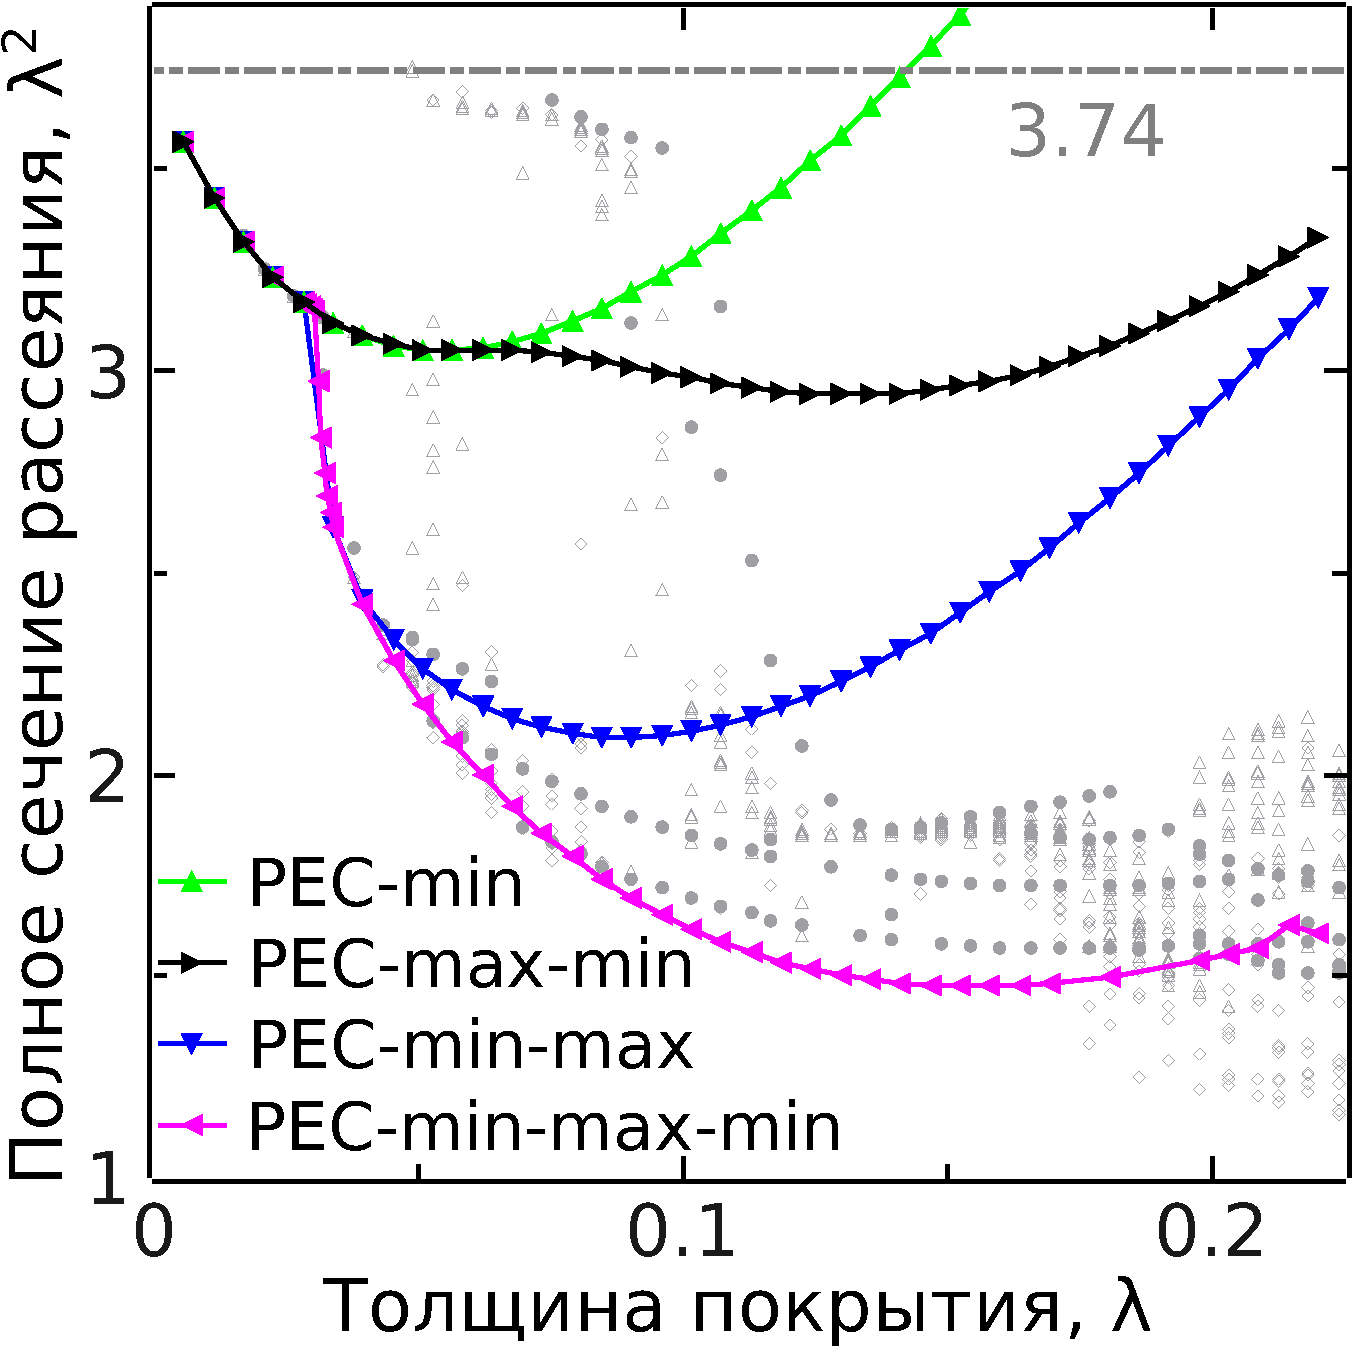
\includegraphics[width=0.95\linewidth]{rcs-overview-index07-DI} \\ а)}
  \end{minipage}
  \hfill
  \begin{minipage}[ht]{0.49\linewidth}
    \center{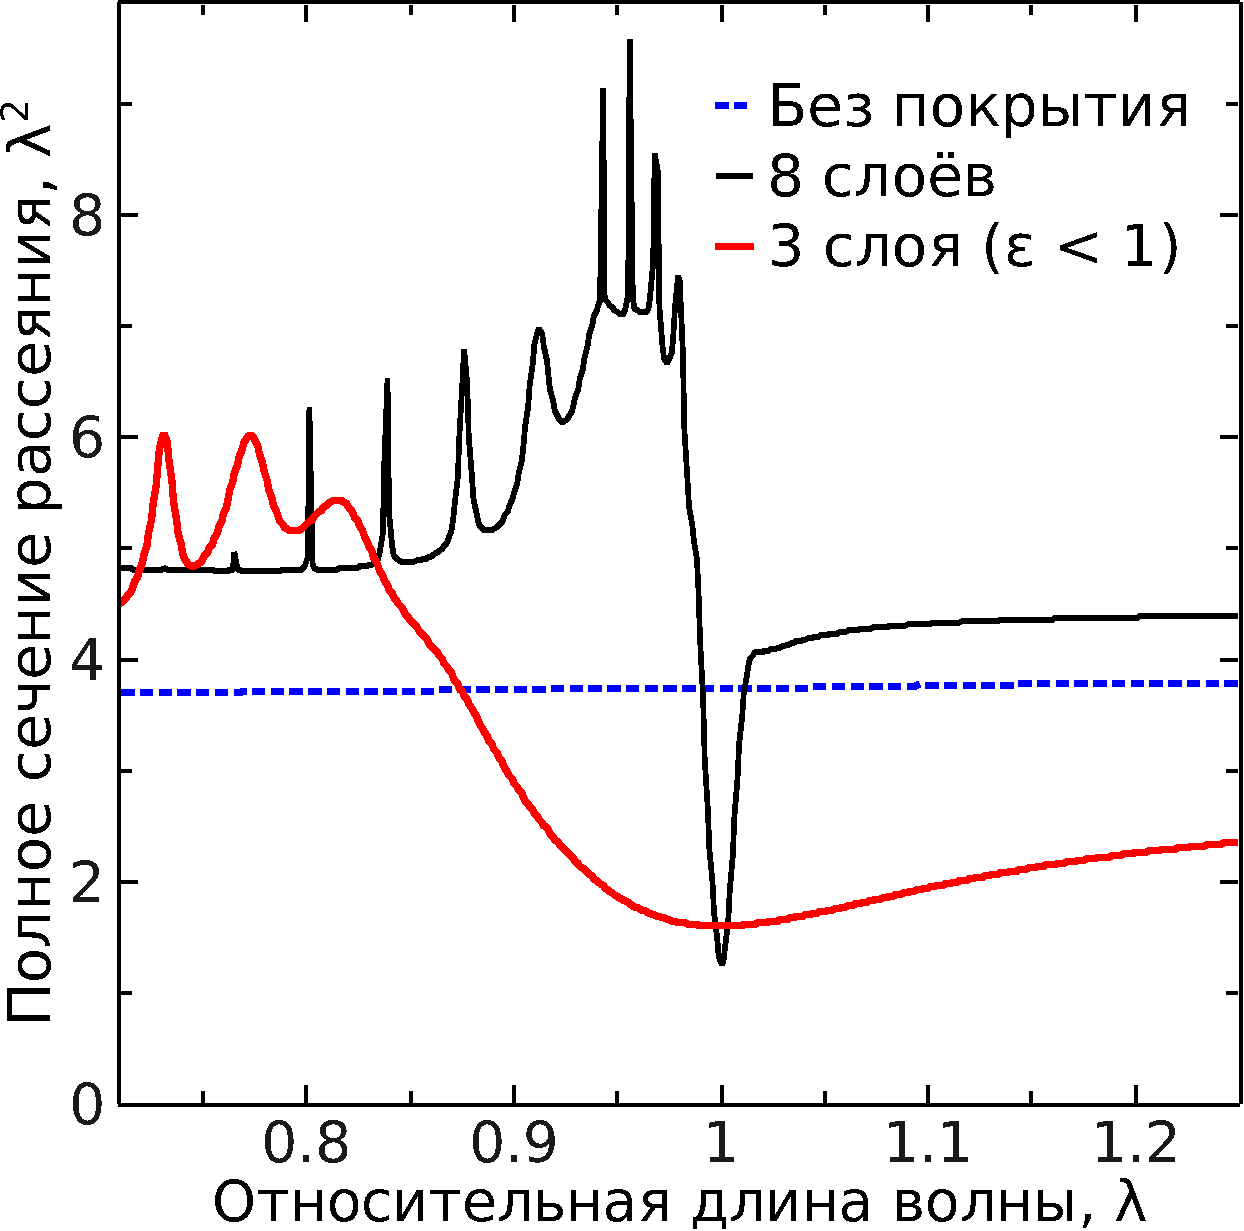
\includegraphics[width=0.95\linewidth]{index07-spectra} \\ б)}
  \end{minipage}
  \caption{а) Результат оптимизации покрытий с чередующимися слоями из
    большого $\varepsilon$ и ${\varepsilon<1}$. б) Спектры частицы
  без покрытия и с маскирующими покрытиями: из 8-ми слоёв диэлектрика и
  из 3-х слоёв с применением ${\varepsilon<1}$.}
  \label{img:min-max-min}  
\end{figure}

Обнаруженная закономерность позволила сформулировать гипотезу о том,
что для создания маскирующего покрытия достаточно использовать всего
два материала: с большим $\varepsilon$ и ${\varepsilon<1}$, а в
качестве параметров оптимизации можно использовать толщину каждого
слоя. Эта гипотеза была проверена численно, результаты оптимизации
отображены на рисунке~\ref{img:min-max-min}а. Оказалось, что для
большей части рассматриваемого диапазона общей толщины покрытия 
достаточно всего трёх слоёв, чтобы получить приблизительно то же
уменьшение полного сечения рассеяния, что и в случае применения 4, 8 и
16 слоёв равной толщины, когда в качестве параметров оптимизации
использовались материальные параметры каждого слоя.

Особый интерес представляет различие в спектрах рассеяния для случаев
наличия и отсутствия материала с ${\varepsilon<1}$ в оптимизированном
покрытии.  При расчёте спектров для рисунка~\ref{img:min-max-min}б не
учитывалось наличие в материалах дисперсии и сопутствующих потерь,
поэтому их форма полностью определяется дизайном маскирующего
покрытия. Хорошо виден относительно узкий резонанс, который определяет
маскирующие свойства покрытия на основе диэлектриков. Использование
материала с ${\varepsilon<1}$ позволило в несколько раз расширить
диапазон длин волн, где наблюдается подавление рассеяния. 

\clearpage